\chapter{引言}

\section{研究的意义及实用价值}

股票市场在我国金融体系中扮演重要的组成部分,反映国民经济的发展水平,为经济发展提供了不可或缺的动力。股票市场的预测、分析对于经济发展也具有重要意义。现有的有效市场理论并不能对一些异常现象进行很好地解释,但随着行为金融理论的提出,人们渐渐意识到投资者的心理和行为都会对股票市场的波动产生重大的影响。

随着互联网的发展,人们越来越多地依赖于网络作为日常生活的场所。在金融领域,互联网也逐渐发挥重要的作用。互联网改变了投资者参与投资活动的方式,也成为主要的投资信息传播的渠道。大众投资者的心理和行为信息,都能够从他们在互联网上的言论中获得分析出来。众多研究表明股票评论并非毫无意义,而是蕴含着大量股票市场的相关信息。因此,挖掘这些相关情绪和信息,帮助投资者优化投资决策,有着重要的现实意义,也是本文的主要研究内容。

\section{研究背景}

经典证券理论认为市场参与者是完全理性的,这样市场价格就在真实价值周围波动,保持稳定。但是,投资者情绪在股票市场中发挥重要的作用,例如“噪声交易者”会因为价值以为的因素交易而产生深远影响。这些行为受到经济学家广泛关注,例如 John Maynard Keynes 在解释股市异常的时候将其比喻为“兽性”, Hume 称之为“激情推动”。相应地,股票市场中的高度投机行为造成了1929年的股票市场爆炸,或者互联网泡沫的发生,而这些现象都很难由简单的基础理论解释。

和经典的完全理性模型相不同,许多新的行为模型试图合理解释发生的这些剧烈波动。 De Long 等人形式化描述了非完全理性(噪声)交易者在市场中扮演的角色。在他们的模型中,有两类投资者:理性套利者和噪声交易者。理性套利者对资产的未来回报持有理性分析,而噪声交易者受外在情感驱动,产生相对于理性分析要么过于乐观要么过于悲观的期待。最终平衡的市场价格反应理性套利者和噪声交易者双方的期待。本质上, De Long 等人证明了市场价格因为不理性的乐观情绪或者悲观情绪会偏离价值,证明了噪声交易者在交易中起到的作用。

在 De Long 等人的工作之后,又有大量的经验文献试图研究投资者情绪及其产生的效果之间的关系。一般人们更多研究情绪直接或者间接的影响。 Lee, Schleifer 和 Thaler 采用基于市场的简介的方式,他们使用了 CEFD 作为投资者情绪的指标,指出 CEFD 是个人情绪积极或者消极和普遍市场情绪的关系。

\section{本文研究内容}

本文的主要研究内容为通过互联网论坛上的股民言论及相关活动信息,试图提取出影响股票市场波动的主要因素。研究股票论坛数据和股票指标变量之间的相互影响关系。试图建立股票成交量和价格的预测模型,对股票市场走势进行预测。

\section{理论背景?}

情感分析理论基础?放到研究背景部分?

\chapter{数据框架}

\section{数据收集、获取}

本文主要研究对象是活跃度较高的股票论坛的关注度数据,其中包含股票评论、访问量的数量和情感倾向。在相类似的研究中,大多采用了如雅虎、 Twitter 、或者新浪财经这样的大型网站,东方财富网和金融界等专门提供财经类信息的网站也有大量关于股票市场的关注度数据。

根据网站活跃度和垃圾信息比例等因素,考虑到大型门户网站在用户交流上有一定的局限性,而太小型的论坛又缺乏信息流通度和有效性,最终选取访问量、人均页面浏览量都很大的股吧,综合考虑选取东方财富网股吧作为主要信息来源。股吧在财经版块设置了新闻、研报和公告等多个版块,针对热门主题和热门个股都有专门的讨论版,信息量充分全面,而且有很好的已经分好类的模块,从各方面都满足本文的需求。

本文另从国信证券金太阳网上交易客户端获取股票市场的交易数据,主要包括个股的开盘价、收盘价、最高价、最低价、成交量以及成交额等。

为了排除掉小众个股非统计性的波动因素,以及可能的人为操控因素,选定上证50成分股作为主要研究对象。上证50成分股有充分的股民和资金来源,能够排除个别资本控盘的非有效市场情况出现。上证50成分股又能从一定程度上反映大盘情况,有重要的研究价值和意义。

东方财富网股吧作为主要的股票市场关注度信息来源,提供活跃度分析及情感分析的重要指标。获取上证50成分股个股论坛的数据,为了简单明确起见,抓取所有讨论帖的标题和浏览量、评论量、发表日期。注意到讨论区里并不完全都是讨论帖,有很多公告、新闻类型的帖子,这些帖子一般都是全论坛共享或是强制置顶的,对于个股差异没有共享,反而会干扰后续阶段的分析,必须注意剔除这些干扰数据。讨论帖的标题可以作为情感分析的原始材料,讨论帖的浏览量和评论量能作为活跃度分析的原始材料,而讨论帖的发表日期可以作为讨论帖的时间戳。严格意义上讨论帖的发表日期不一定是所有活跃度发生的日期,但是考虑到论坛日均流量很大,老帖很快就会掉出首页,可以粗略认为讨论帖的发表日期即为活跃度发生的时间。由统计上的随机性也可以做出类似的论断,最终活跃度的期望是不受此时间差的影响的。

在实际抓取活跃度数据过程中,发现东方财富网股吧为手机端网页提供了 RESTful API 接口 http://m.guba.eastmoney.com/getdata/articlelist 。可以发送 GET 请求,参数 code 指定股票代码,参数 count 指定返回条数的个数,上限为 200 ,参数 thispage 指定当前页码。即可以固定 count 为 200 ,依次获取每页的所有评论信息,直到服务器返回空值为之,代表已经处理完所有的评论。因为抓取数据的过程中可能有事实的新数据产生,为了防止新帖的出现导致整体向后位移干扰抓取结果,可以按照从前往后的顺序抓取,这样至多抓到重复数据,而不会漏抓。

服务器正常返回的数据结构如下所示。

; Code snippet here
; 瞎鸡巴说一通

考虑到获取数据的部分主要都是网络 I/O ,所以是访存密集型而不是计算密集型的任务。决定采用 Node.js 框架编写程序。 Node.js 原生带有事件循环机制,对于异步任务的支持非常地好,再加上外部 promise 库,可以发挥显著的作用。在实际中测试,利用异步 HTTP 请求,能在单核的情况下跑满所有网络带宽,达到性能上的极限。 获取服务器请求的程序逻辑如下。

; Code snippet here

获取的结果放入 Redis 数据库中,同样也是异步地完成。考虑到获取原始数据的过程中可能发生各种不可预料的网络临时故障或解析错误,此时应该尽早抛出错误,使得程序异常退出,使用外部稳定的数据库可以保证不会丢失数据。 股票市场价格和交易量数据通过国信证券金太阳网上交易客户端获取,该客户端可以到处历史数据成 CSV 格式文件。

至此所有原始数据已经获取完毕。

\section{数据预处理}

为了提取出讨论帖的情感因素,需要用到自然语义分析和情感分析的工具。对于英文的文本分析已经比较成熟了,但对于中文的语义分析还停留在比较表面的阶段。最简单的办法是根据积极情感和消极情感制作两个词表,然后根据词表的匹配程度来决定积极情感和消极情感的明显程度。但是比较开源的已有的中文词表之后发现,大部分词表被没有针对股票市场的特定应用环境,所以很多在股票论坛里带有强烈情感色彩的词语都没有被收录, 比如“大涨”、“大跌”都是很常见的极性很强的情感词语。

为了解决词表不够精确的问题,必须修改已有的情感分析模型以适应新的任务。可以利用 GitHub 上的开源项目 twitter-sent-dnn (https://github.com/xiaohan2012/twitter-sent-dnn) 。这是一个利用卷积神经网络,利用 Twitter 数据作为训练集训练得到的分析英语短文情感的模型。使用深度卷积神经网络的好处在于可以挖掘句子内词语之间的复杂的逻辑关系,得到深层的语义上的信息。具体来说,这个模型使用了 Twitter140 的数据作为训练数据。此数据源包含约 160 万已标注的 Twitter 数据供训练使用。在训练数据中,标注的方式是自动进行的,根据 Twitter 中的表情符号作为标注的基准,得到积极情感和消极情感的极性参数。最后去除这些表情符号,作为真正的训练输入。此数据集另有 872 条验证数据和 1821 条测试数据。这两种数据是人工标注的。除此之外,此模型还使用了实时的 Twitter 数据流作为训练数据。

为了把此模型应用在之前抓取的东方财富网股吧数据上,还需解决语言的映射问题。如果直接将中文通过机器翻译变成英文,一般情况下是会保留词语的意思和情感极性,但是会打乱句子的结构。不过在此情感模型的情况下,这并不会造成很大的影响。考虑到此情感模型是基于 Twitter 训练的。 Twitter 数据大多是短小破碎的语句,精简但蕴含强烈的语言情感。所以直接通过机器翻译将中文翻译成英文,再通过此情感模型,即可得到较好的结果。

Demo here
在这里,翻译使用了百度翻译 API 。至本论文成文之时,百度宣布即将发布新的基于深度神经网络的翻译模型,但是并未公开其 API ,所以本文所使用的百度翻译 API 均为现有模型。

基于下面代码逻辑,实现百度翻译 API 的自动调用。

; code snippet here
; describe how it works, how it achieves parallelism, flow control, error control

基于上述操作,简单地搭建出了实验需要用到的语言情感模型。简单地测试一下,可以发现其性能完全满足情感极性分析的要求。

; Demo here

最后通过一些黏合脚本,将数据导入预处理阶段,并且将处理后的数据序列化成 JSON 格式以供后续阶段分析。部分代码逻辑如下所示。

; code snippet here

; extract final usable data, read count and volume

\chapter{成交量与情绪的关系}

\section{格兰杰因果关系}

格兰杰因果关系检验\cite{granger_causality}是一种假设检验的统计方法,检验一组时间序列 $x$ 是否为另一组时间序列 $y$ 的原因。回归分析通常只能得出不同变量间的同期相关性,自回归模型只能得出同一变量前两前后期的相关性,但格兰杰证明了在自回归模型中通过一系列的检验而揭示不同变量之间的时间落差相关性是可行的。需要注意的是,这里所说的原因,抑或时间落差相关性,并无法证明逻辑意义上的因果关系,只能从时间现在的关系上解释过去发生的事件对以后发生的事件有预测作用。

格兰杰因果关系检验的核心假设在于,未来的事件不会对目前和过去的事件产生影响,而过去
的事件才可能对现在及未来产生影响。假如在控制了时间序列 $y$ 的过去值以后,时间序列 $x$ 的过去值仍能对时间序列 $y$ 有显著的解释能力,就意味着 $x$ 能格兰杰影响 $y$ 。

它的严格数学定义如下。令 $x$ 和 $y$ 为广义平稳序列。如果要检验 $x$ 非 $y$ 的格兰杰原因之零假设,首先引入 $y$ 的落后期建立 $y$ 的自回归模型如下。

\begin{equation}
  \label{granger:0}
  y_{t}=a_{0}+a_{1}y_{t-1}+a_{2}y_{t-2}+\cdots+a_{m}y_{t-m}+residual_{t}.
\end{equation}

简单表示即为

\begin{equation}
  \label{granger:1}
  y_{t}=a_{0}+\sum_{i=1}^{m}a_{i}y_{t-i}+residual_{t}.
\end{equation}

式 \ref{granger:0} 和式 \ref{granger:1} 中的 $m$ 即为落后期。在落后期固定的情况下,使得 $residual$ 极大似然正态分布的系数序列 $a_{i}$ ,同时为使得预测值

\begin{equation}
  \label{granger:2}
  \hat{y}_{t}=a_{0}+\sum_{i=1}^{m}a_{i}y_{t-i}
\end{equation}
与标准值 $y_{t}$ 的 $L_{2}$ 范数最小的系数序列。取此系数得到自回归模型同式 \ref{granger:2} 。

接着引入 $x$ 的落后期建立增广回归模型如下。

\begin{equation}
  \label{granger:3}
  y_{t}=a_{0}+\sum_{i=1}^{m}a_{i}y_{t-i}+\sum_{i=1}^{m}b_{i}x_{t-i}+residual_{t}.
\end{equation}

同样的方法可以得到系数序列 $b_{i}$ 。

如果没有任何 $x$ 的落后期被留在模型中,即可以定性地认为从某种意义上 $b_{i}=0$
对于所有的 ${i}$ 都成立,无格兰杰因果关系的零假设成立。

\section{落后期计算方法}

计算时间序列 $x$ 的落后期,可以使用多种方法。在本文中,主要使用以下四种方法。

\begin{enumerate}
  \item Akaike information criterion
  \item Bayesian information criterion
  \item Final prediction error
  \item Hannan-Quinn information criterion
\end{enumerate}

其中 Bayesian information criterion 也被称作 Schwarz criterion 。这些选取落后期
的模型本身之间差别并不明显,但是在某些情况下会给出不同的选取结果。

Bayesian information criterion 的定义如下。

\begin{equation}
  \label{bic:0}
  \text{BIC}=-2\cdot \ln \hat{L}+k\cdot \ln n.
\end{equation}

在式 \ref{bic:0} 中, $\hat{L}$ 为模型 $M$ 似然性方程的最大值,如果令 $\hat{\theta}$ 为取得极大似然性的参数,则

\begin{equation}
  \label{bic:1}
  \hat{L}=p(x\mid \hat{\theta},M).
\end{equation}

在式 \ref{bic:0} 中, $n$ 为数据点的个数, $k$ 为自由变量的个数。

直观上可以理解, $-2\cdot \ln \hat{L}$ 项使得模型尽可能拟合,这就要求落后期越大越好,而 $k\cdot \ln n$ 项使得模型不是很大,防止过拟合的情况出现。其他几种选取落后期的方法本质上大同小异,不再详细介绍。

\section{落后期计算}

不妨尝试建立基于成交量和讨论贴点击量的向量自回归模型,本文使用了 Python 的数据挖掘框架 Statsmodels\cite{statsmodels} 。该框架对于成熟的线性和非线性数据模型都有准确高效的实现,并且自带简单的画图功能。取浦发银行 (600000) 在 2012 年 5 月 1 日至 2015 年 4 月 1  日之间的过往成交量和对应日期的讨论帖点击量,如图 \ref{auto_regression:0} 所示。

\begin{figure}
  \centering
  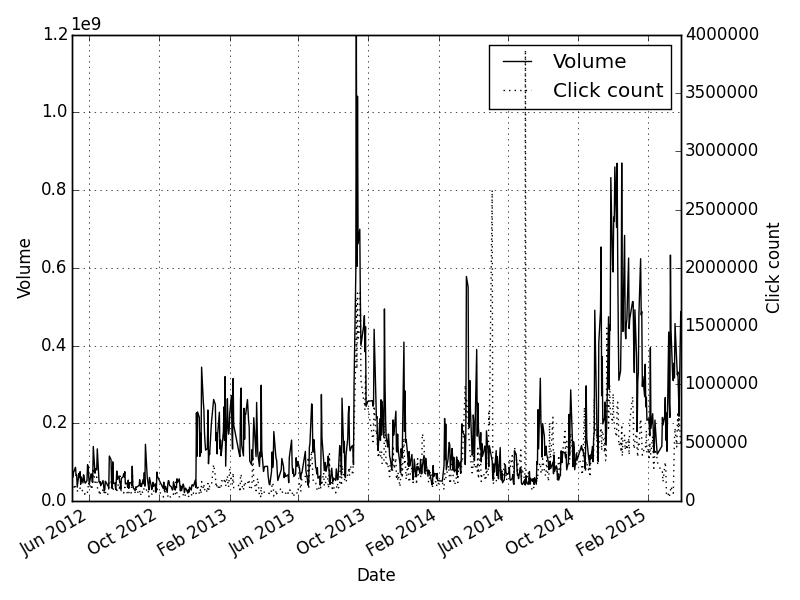
\includegraphics[width=0.9\textwidth]{plots/auto_regression_0.png}
  \caption{浦发银行 (600000) 成交量}
  \label{auto_regression:0}
\end{figure}

建立向量自回归模型,根据参数选取最佳落后期,见代码 \ref{auto_regression:2} 。落后期选择的结果见表 \ref{auto_regression:1} 。标星的数据表示最优的选择。可见根据 AIC 和 FPE 标准,最佳落后期是 $4$ ,而按照 BIC 标准,最佳落后期是 $2$ 。按照 HQIC ,最佳落后期是 $3$ 。在本文中,鉴于模型的特性,默认情况下使用 HQIC 作为落后期选择的方法。

\begin{table}
  \centering
  \caption{落后期选择}
  \label{auto_regression:1}
  \begin{tabularx}{0.75\textwidth}{XXXXX}
    \toprule
    & AIC & BIC & FPE & HQIC \\
    \midrule
    0 & 62.45 & 62.46 & 1.324e+27 & 62.46 \\
    1 & 61.23 & 61.27 & 3.894e+26 & 61.24 \\
    2 & 61.08 & 61.15* & 3.366e+26 & 61.11 \\
    3 & 61.07 & 61.16 & 3.322e+26 & 61.10* \\
    4 & 61.06* & 61.18 & 3.311e+26* & 61.11 \\
    5 & 61.07 & 61.21 & 3.324e+26 & 61.12 \\
    6 & 61.07 & 61.24 & 3.325e+26 & 61.14 \\
    7 & 61.07 & 61.27 & 3.334e+26 & 61.15 \\
    8 & 61.08 & 61.30 & 3.358e+26 & 61.17 \\
    9 & 61.09 & 61.34 & 3.393e+26 & 61.19 \\
    10 & 61.10 & 61.38 & 3.423e+26 & 61.21 \\
    11 & 61.10 & 61.41 & 3.445e+26 & 61.22 \\
    12 & 61.11 & 61.44 & 3.478e+26 & 61.24 \\
    13 & 61.12 & 61.47 & 3.489e+26 & 61.26 \\
    14 & 61.13 & 61.51 & 3.526e+26 & 61.28 \\
    15 & 61.14 & 61.55 & 3.554e+26 & 61.29 \\
    16 & 61.14 & 61.58 & 3.574e+26 & 61.31 \\
    17 & 61.15 & 61.61 & 3.611e+26 & 61.33 \\
    18 & 61.15 & 61.64 & 3.592e+26 & 61.34 \\
    19 & 61.16 & 61.67 & 3.631e+26 & 61.36 \\
    20 & 61.16 & 61.70 & 3.649e+26 & 61.37 \\
    \bottomrule
  \end{tabularx}
\end{table}

\begin{figure}
  \begin{minipage}{\textwidth}
    \begin{lstlisting}[caption=落后期选择逻辑, label=auto_regression:2]
data = pandas.DataFrame({'volume': volume,
  'clickCount': click_count})
data.index = pandas.DatetimeIndex(dates)
model = statsmodels.tsa.api.VAR(data)
    \end{lstlisting}
  \end{minipage}
\end{figure}

\section{假设检验方法}

为了检验 $x$ 对 $y$ 的格兰杰因果关系,需要检验 $y$ 的相量自回归模型中没有 $x$ 的过去值的影响。需要检验向量自回归模型中 $x$ 的系数的大小。回顾格兰杰因果关系模型如式 \ref{null_hypothesis:0} 所示,可以做出零假设 $x$ 对 $y$ 并没有格兰杰因果关系,如式 \ref{null_hypothesis:1}所示。

\begin{equation}
  \label{null_hypothesis:0}
  y_{t}=a_{0}+\sum_{i=1}^{m}a_{i}y_{t-i}+\sum_{i=1}^{m}b_{i}x_{t-i}+residual_{t}.
\end{equation}

\begin{equation}
  \label{null_hypothesis:1}
  H_{0}:b_{1}=b_{2}=\cdots =b_{m}=0
\end{equation}

而拒绝假设 $H_{0}$ 意味着 $x$ 对 $y$ 有格兰杰因果关系。

在 Statsmodels 的实现里,一共使用了四种方法进行假设检验。

\begin{enumerate}
  \item 参数 $F$ 检验
  \item 残差平方和 $F$ 检验
  \item 残差平方和 $\chi^{2}$ 检验
  \item 似然比检验
\end{enumerate}

以残差平方和 $F$ 检验为例,步骤如下。

首先得到约束方程如式 \ref{f_test:0} 的最小二乘解。

\begin{equation}
  \label{f_test:0}
  y_t=a_{0}+\sum_{i=1}^{m}a_{i}y_{t-i}+e_{t}.
\end{equation}

代入最小二乘解得到自回归模型如式 \ref{f_test:1} 。

\begin{equation}
  \label{f_test:1}
  \hat{y}_t=a_{0}+\sum_{i=1}^{m}a_{i}y_{t-i}.
\end{equation}

利用自回归模型得到残差如式 \ref{f_test:2} 。

\begin{equation}
  \label{f_test:2}
  \hat{e}_t=y_{t}-\hat{y}_t.
\end{equation}

最后得到残差平方和如式 \ref{f_test:3} 。

\begin{equation}
  \label{f_test:3}
  RSS_{0}=\sum_{i=1}^{m}\hat{e}_{t}^2.
\end{equation}

使用同样的方法,处理非约束方程如式 \ref{f_test:4} 所示,得到非约束方程的残差平方和如式 \ref{f_test:5} 。

\begin{equation}
  \label{f_test:4}
  y_{t}=a_{0}+\sum_{i=1}^{m}a_{i}y_{t-i}+\sum_{i=1}^{m}b_{i}x_{t-i}+u_{t}.
\end{equation}

\begin{equation}
  \label{f_test:5}
  RSS_{1}=\sum_{i=1}^{m}\hat{u}_{t}^2.
\end{equation}

计算检验统计量如式 \ref{f_test:6} 。

\begin{equation}
  \label{f_test:6}
  S_{1}=\frac{(RSS_{0}-RSS_{1})/p}{RSS_{1}/(m-2p-1)}\sim F_{p,m-2p-1}.
\end{equation}

如果 $S_{1}$ 大于指定的临界值,则拒绝原假设 $H_{0}$ 。

在残差平方和 $\chi^{2}$ 检验中,则最后一步检验统计量如式 \ref{f_test:7} 。

\begin{equation}
  \label{f_test:7}
  S_{1}=\frac{m(RSS_{0}-RSS_{1})}{RSS_{1}}\sim \chi^{2}(p).
\end{equation}

\section{假设检验}

对浦发银行 (600000) 在 2012 年 5 月 1 日至 2015 年 4 月 1 日之间的成交量和对应日期的讨论帖点击量进行格兰杰因果关系检验。程序逻辑如代码 \ref{f_test:8} 所示。基于之前的结果,已经知道最佳落后期为 $3$ ,而在进行格兰杰因果关系检验的时候,需要输入一个最大落后期,然后程序会从 $1$ 到指定的最大落后期都计算统计检验量和对应的 $p$ 值。所以在程序代码中指定最大落后期为 $5$ 。得到输出如代码 \ref{f_test:9} 所示。

\begin{figure}
  \begin{minipage}{\textwidth}
    \begin{lstlisting}[caption=浦发银行 (600000) 格兰杰因果关系检验, label=f_test:8]
statsmodels.tsa.api.stattools.\
grangercausalitytests(d, 5, verbose=True)
    \end{lstlisting}
  \end{minipage}
\end{figure}

\begin{figure}
  \begin{minipage}{\textwidth}
    \begin{lstlisting}[caption=浦发银行 (600000) 检验结果, label=f_test:9]
Granger Causality
number of lags (no zero) 1
ssr based F test:         F=16.3569 , p=0.0001  , df_denom=701, df_num=1
ssr based chi2 test:   chi2=16.4269 , p=0.0001  , df=1
likelihood ratio test: chi2=16.2382 , p=0.0001  , df=1
parameter F test:         F=16.3569 , p=0.0001  , df_denom=701, df_num=1


Granger Causality
number of lags (no zero) 2
ssr based F test:         F=3.9950  , p=0.0188  , df_denom=698, df_num=2
ssr based chi2 test:   chi2=8.0472  , p=0.0179  , df=2
likelihood ratio test: chi2=8.0015  , p=0.0183  , df=2
parameter F test:         F=3.9950  , p=0.0188  , df_denom=698, df_num=2


Granger Causality
number of lags (no zero) 3
ssr based F test:         F=2.9458  , p=0.0322  , df_denom=695, df_num=3
ssr based chi2 test:   chi2=8.9265  , p=0.0303  , df=3
likelihood ratio test: chi2=8.8702  , p=0.0311  , df=3
parameter F test:         F=2.9458  , p=0.0322  , df_denom=695, df_num=3


Granger Causality
number of lags (no zero) 4
ssr based F test:         F=2.3264  , p=0.0550  , df_denom=692, df_num=4
ssr based chi2 test:   chi2=9.4267  , p=0.0513  , df=4
likelihood ratio test: chi2=9.3638  , p=0.0526  , df=4
parameter F test:         F=2.3264  , p=0.0550  , df_denom=692, df_num=4


Granger Causality
number of lags (no zero) 5
ssr based F test:         F=2.1061  , p=0.0629  , df_denom=689, df_num=5
ssr based chi2 test:   chi2=10.6987 , p=0.0577  , df=5
likelihood ratio test: chi2=10.6178 , p=0.0595  , df=5
parameter F test:         F=2.1061  , p=0.0629  , df_denom=689, df_num=5
    \end{lstlisting}
  \end{minipage}
\end{figure}

分析格兰杰因果关系检验中假设检验的结果,其中 $p$ 值随落后期的变化如表 \ref{f_test:10} 和图 \ref{f_test:11} 所示。理所应当地,随着落后期的增加,成交量自己携带的信息量越来越大,对于点击量信息量的依赖越来越小, $p$ 值单调递增。但是这并不是绝对的规律,因为成交量和点击量都会携带越来越多的信息,要根据最佳落后期实际情况变化来分析 $p$ 值的变化。如果选择显著性水平 $\alpha=0.05$ ,则在落后期为之前已经选择的最佳落后期 $3$ 的时候就已经可以拒绝零假设 $H_{0}$ ,认为讨论帖点击量对于成交量有格兰杰因果关系。

\begin{table}
  \centering
  \caption{浦发银行 (600000) 格兰杰因果关系检验 $p$ 值}
  \label{f_test:10}
  \begin{tabular}{rrrrr}
    \toprule
    落后期 & SSR $\chi^{2}$ test & Params $F$ test & LR $\chi^{2}$ test & SSR $F$ test \\
    \midrule
    1 & 0.0001 & 0.0001 & 0.0001 & 0.0001 \\
    2 & 0.0188 & 0.0179 & 0.0183 & 0.0188 \\
    3 & 0.0322 & 0.0303 & 0.0311 & 0.0322 \\
    4 & 0.0550 & 0.0513 & 0.0526 & 0.0550 \\
    5 & 0.0629 & 0.0577 & 0.0595 & 0.0629 \\
    \bottomrule
  \end{tabular}
\end{table}

\begin{figure}
  \centering
  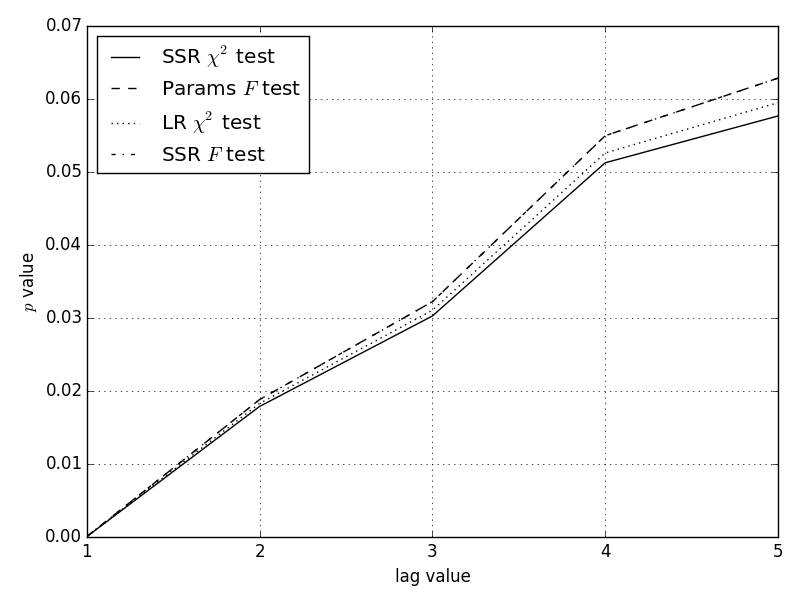
\includegraphics[width=0.8\textwidth]{plots/granger_causality_test_1.png}
  \caption{浦发银行 (600000) 格兰杰因果关系检验 $p$ 值}
  \label{f_test:11}
\end{figure}

不妨对于上证 50 所有股票进行格兰杰因果关系检验。使用同样的方法计算 50 支股票的四种检验下的 $p$ 值。结果如下所示。

\begin{enumerate}
  \item 似然比检验结果如图 \ref{f_test:12} 所示
  \item 参数 $F$ 检验结果如图 \ref{f_test:13} 所示
  \item 残差平方和 $\chi^{2}$ 检验结果如图 \ref{f_test:14} 所示
  \item 残差平方和 $F$ 检验结果如图 \ref{f_test:15} 所示
\end{enumerate}

可以发现有如下几条规律。首先对于某一特定股票而言,四种检验方法的差别并不是很大,从对于零假设 $H_{0}$ 的验证的角度来说是没有区别的。从一个角度上增加了结果的可信度。其次不妨取显著性水平 $\alpha=0.05$ ,在这种情况下,大部分股票都能得出拒绝零假设的结论。 50 支股票中只有 9 支股票是认为讨论帖点击量对于成交量是没有格兰杰因果关系的,其他 41 支股票都是有关系的。从理论上证明了这种格兰杰因果关系的普遍性。关于这 9 支股票的特殊情况,可能有以下几种可能。

\begin{enumerate}
  \item 该股票本身存在异常情况,不符合普遍规律,例如受到庄家操控等人为因素影响
  \item 该股票讨论区存在比较极端的讨论帖,干扰统一分析格兰杰因果关系
\end{enumerate}

对于第二种情况,在格兰杰因果关系中某些数据点出现的异常值能很敏感地影响假设检验的结果。例如有些之前的讨论帖被频繁顶至首页,导致总点击量很高。但是这些点击量并不如在数据框架中所假设的是短时间内产生的,而是长时间的积累,但这些点击量都被计入讨论帖发帖日期的点击量上。这样的数据点即使只有两三个,也会对检验结果造成比较深刻的影响。为解决这些问题,数据的预处理显得尤为关键如何辨别并且抹平这些极端数据点,但是又不忽视正常情况下出现的极大极小值,是非常细节并且值得深入探讨的。

\begin{figure}
  \centering
  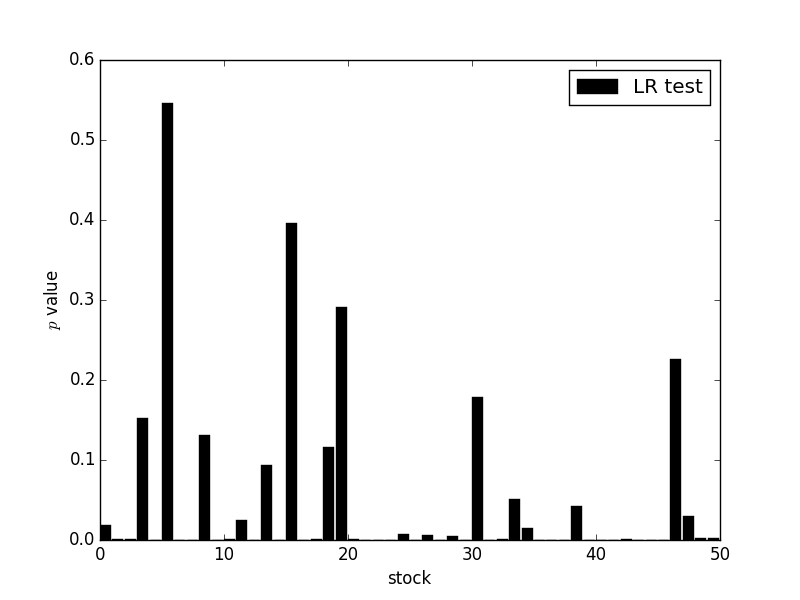
\includegraphics[width=0.9\textwidth]{plots/granger_causality_test_on_sse_50_lrtest.png}
  \caption{上证 50 似然比检验}
  \label{f_test:12}
\end{figure}

\begin{figure}
  \centering
  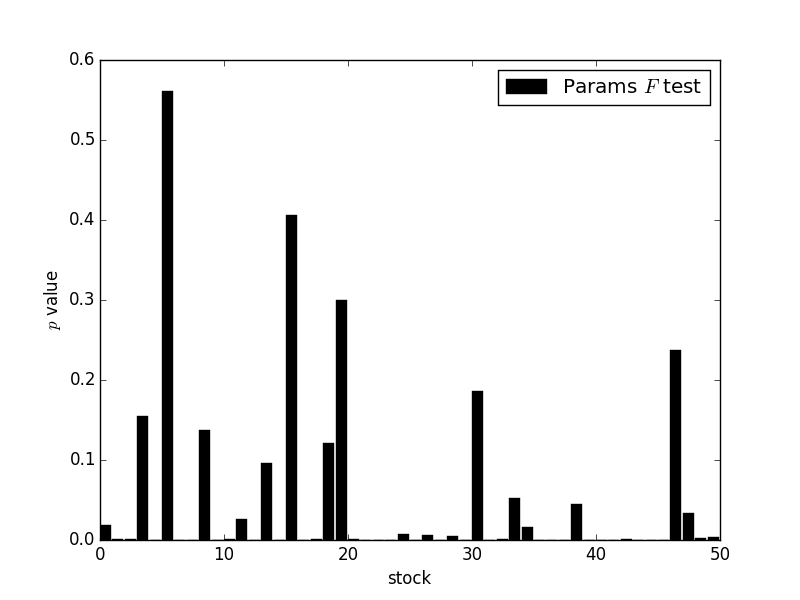
\includegraphics[width=0.9\textwidth]{plots/granger_causality_test_on_sse_50_params_ftest.png}
  \caption{上证 50 参数 $F$ 检验}
  \label{f_test:13}
\end{figure}

\begin{figure}
  \centering
  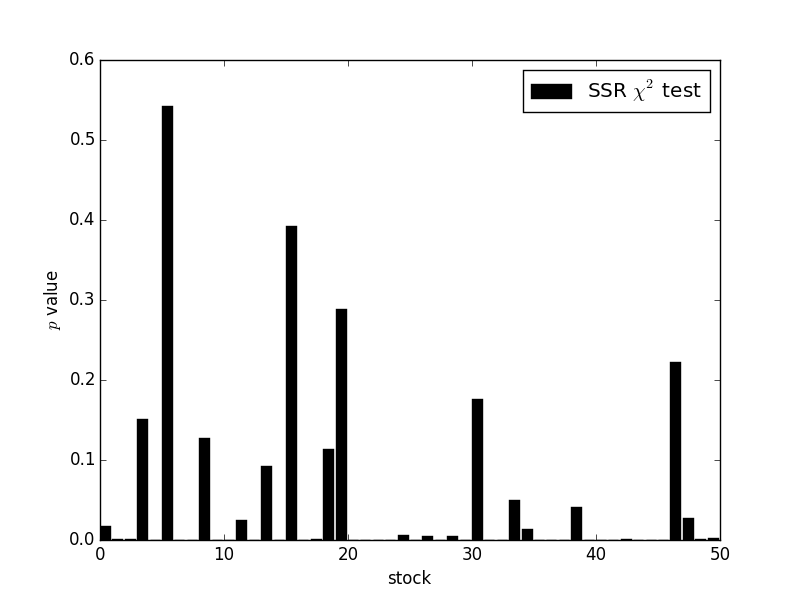
\includegraphics[width=0.9\textwidth]{plots/granger_causality_test_on_sse_50_ssr_chi2test.png}
  \caption{上证 50 残差平方和 $\chi^{2}$ 检验}
  \label{f_test:14}
\end{figure}

\begin{figure}
  \centering
  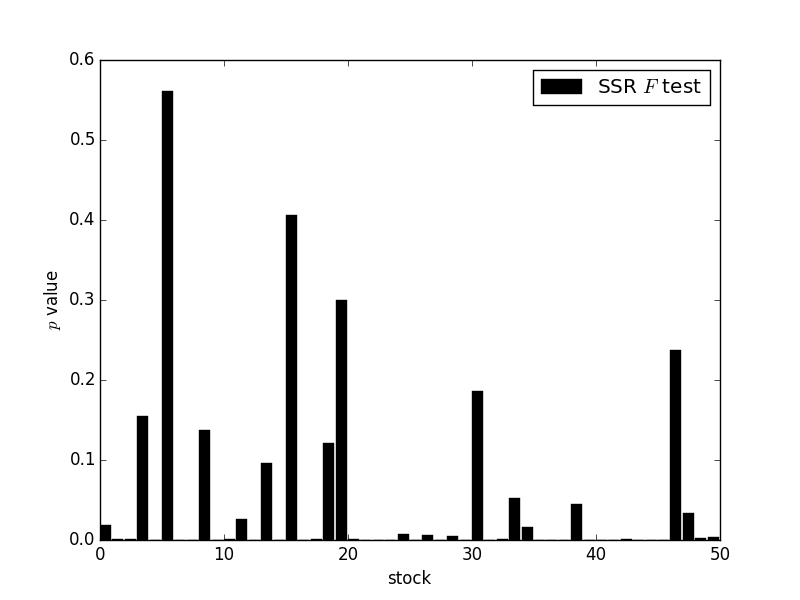
\includegraphics[width=0.9\textwidth]{plots/granger_causality_test_on_sse_50_ssr_ftest.png}
  \caption{上证 50 残差平方和 $F$ 检验}
  \label{f_test:15}
\end{figure}

需要注意的是,在格兰杰因果检验的过程中,落后期的选择十分重要。对于同一支股票,落后期的不同会导致假设检验得到的 $p$ 值产生很大的不同。可以理解的是落后期的不同使得讨论帖点击量带来的影响的作用产生极大的分歧。所以选择对的落后期是格兰杰因果关系检验的关键。

而且之所以如此关注落后期的选择,因为一个足够精简的模型是十分必要的。选择过大的落后期会导致模型模拟和,对于后续的预测和分析是十分不利地。

\section{异常分析}

不妨单独观察 $p$ 值最高的股票中国石化 (600028) 。其落后期的选择如表 \ref{granger_causality_test_on_sse_50_abnormal:0} 所示。显而易见的是四种落后期选择的指标产生了极大的分歧,预示着此数据带来的不对称性使得落后期的选择不稳定。

\begin{table}
  \centering
  \caption{中国石化 (600028) 落后期选择}
  \label{granger_causality_test_on_sse_50_abnormal:0}
  \begin{tabularx}{0.75\textwidth}{XXXXX}
    \toprule
    & AIC & BIC & FPE & HQIC \\
    \midrule
      0 & 61.60 & 61.61 & 5.661e+26 & 61.61 \\
      1 & 59.68 & 59.72 & 8.286e+25 & 59.69 \\
      2 & 59.60 & 59.67* & 7.654e+25 & 59.63 \\
      3 & 59.59 & 59.68 & 7.542e+25 & 59.62 \\
      4 & 59.59 & 59.71 & 7.566e+25 & 59.63 \\
      5 & 59.59 & 59.73 & 7.561e+25 & 59.64 \\
      6 & 59.56 & 59.73 & 7.322e+25 & 59.62 \\
      7 & 59.55 & 59.74 & 7.250e+25 & 59.62 \\
      8 & 59.48 & 59.70 & 6.774e+25 & 59.56* \\
      9 & 59.48 & 59.73 & 6.764e+25 & 59.57 \\
      10 & 59.48 & 59.76 & 6.801e+25 & 59.59 \\
      11 & 59.48 & 59.79 & 6.822e+25 & 59.60 \\
      12 & 59.49 & 59.82 & 6.829e+25 & 59.61 \\
      13 & 59.49 & 59.85 & 6.890e+25 & 59.63 \\
      14 & 59.49 & 59.87 & 6.838e+25 & 59.64 \\
      15 & 59.49 & 59.90 & 6.839e+25 & 59.65 \\
      16 & 59.49 & 59.92 & 6.839e+25 & 59.66 \\
      17 & 59.49 & 59.95 & 6.849e+25 & 59.67 \\
      18 & 59.44 & 59.92 & 6.495e+25 & 59.62 \\
      19 & 59.43* & 59.94 & 6.440e+25* & 59.63 \\
      20 & 59.43 & 59.97 & 6.457e+25 & 59.64 \\
    \bottomrule
  \end{tabularx}
\end{table}

得到其格兰杰因果关系检验的 $p$ 值随落后期变化,如图 \ref{granger_causality_test_on_sse_50_abnormal:1} 所示。可以看出其 $p$ 值一直都在 $0.2$ 以上,对于这种极端情况,无论选择什么样的落后期都无法验证其格兰杰因果关系。

\begin{figure}
  \centering
  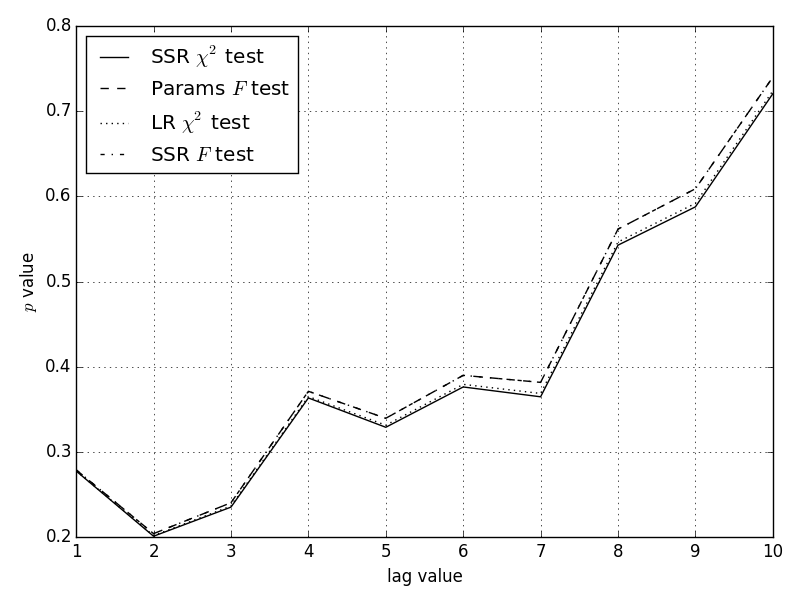
\includegraphics[width=0.9\textwidth]{plots/granger_causality_test_on_sse_50_abnormal_granger.png}
  \caption{中国石化 (600028) 格兰杰因果关系检验 $p$ 值}
  \label{granger_causality_test_on_sse_50_abnormal:1}
\end{figure}

继续深究原因,得到其成交量与讨论帖点击量折线图如图 \ref{granger_causality_test_on_sse_50_abnormal:2} 所示。比较明显的是在 2013 年 8 月左右的时间点,有一次点击量的突然增加,但是并没有对应成交量的大幅度变化。根据之前的分析,有可能是确实讨论区产生了如此异常的反应,也有可能是讨论帖归类的原因导致了过去的老贴被过多累加点击量。至此,可以发现该股票产生异常高的 $p$ 值的直接原因。其他几支 $p$ 值异常的股票也有各自不同的原因,深层次可能有更加统一地解释。但是对于绝大多数股票来说,都是符合格兰杰因果关系检验的结果的,不妨更多关注于普遍情况,利用其格兰杰因果关系。

\begin{figure}
  \centering
  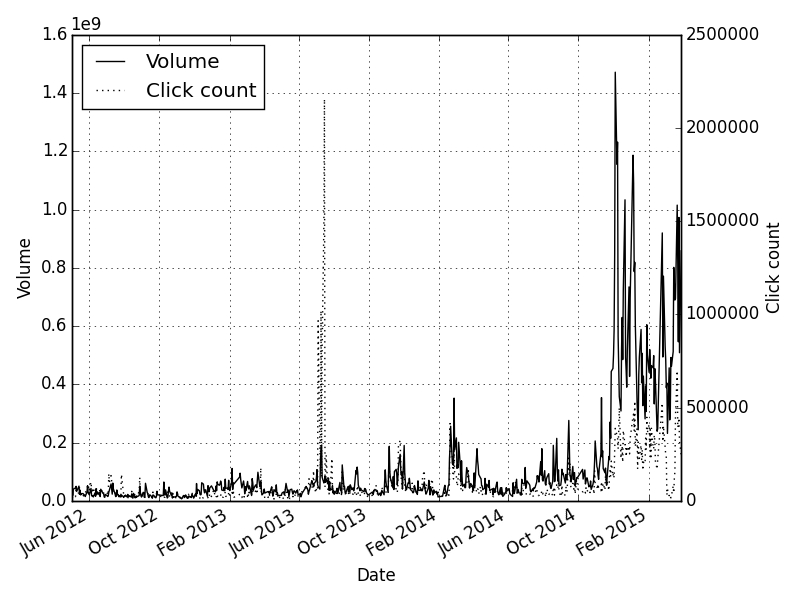
\includegraphics[width=0.9\textwidth]{plots/granger_causality_test_on_sse_50_abnormal_plot.png}
  \caption{中国石化 (600028) 成交量与讨论帖点击量}
  \label{granger_causality_test_on_sse_50_abnormal:2}
\end{figure}

\section{预测模型}

试图利用向量自回归模型做最简单的预测模型。首先给出向量自回归模型的严格构造。它描述了在同一样本期间内的 $n$ 个内生变量可以作为它们过去值的线性函数。可以写成如式 \ref{var:0} 所示。

\begin{equation}
  \label{var:0}
  y_{t}=c+A_{1}y_{t-1}+A_{2}y_{t-2}+\cdots +A_{p}y_{t-p}+e_{t}.
\end{equation}

其中 $c$ 是 $n\times 1$ 的常数向量, $A_{i}$ 是 $n\times n$ 矩阵, $e_{t}$ 是 $n\times 1$ 的误差向量。误差项满足以下几条性质。

\begin{enumerate}
  \item $E(e_{t})=0$
  \item $E(e_{t}e_{t}^{\prime})=\Omega$ (正定矩阵)
  \item $E(e_{t}e_{t-k}^{\prime})=0$
\end{enumerate}

在自回归模型的参数 $A_{i}$ 都已知,并且没有外生变量的情况下,在最小误差平方和的意义下最好的线性预测函数是基于向量自回归模型本身的,进行提前 $1$ 步的预测,即在已有时间 $t$ 信息的基础上预测 $y_{t+1}$ ,如式 \ref{var:1} 所示。

\begin{equation}
  \label{var:1}
  y_{t+1\mid t}=c+A_{1}y_{t}+A_{2}y_{t-1}+\cdots +A_{p}y_{t-p+1}.
\end{equation}

要预测更长的提前量,可以使用预测链式法则,如式 \ref{var:2} 所示。其中当 $j\leq 0$ 的时候 $y_{t+j\mid t}=y_{t+j}$ 。

\begin{equation}
  \label{var:2}
  y_{t+h\mid t}=c+A_{1}y_{t+h-1\mid t}+A_{2}y_{t+h-2\mid t}+\cdots +A_{p}y_{t-p+h\mid t}.
\end{equation}

;; sliding window trick

;; result

;; non-linear models possible

; model construction

; model testing
% Local Variables:
% fill-column: 80
% eval: (flycheck-mode -1)
% eval: (auto-fill-mode 1)
% End: